\begin{figure*}[t]
 \centering
 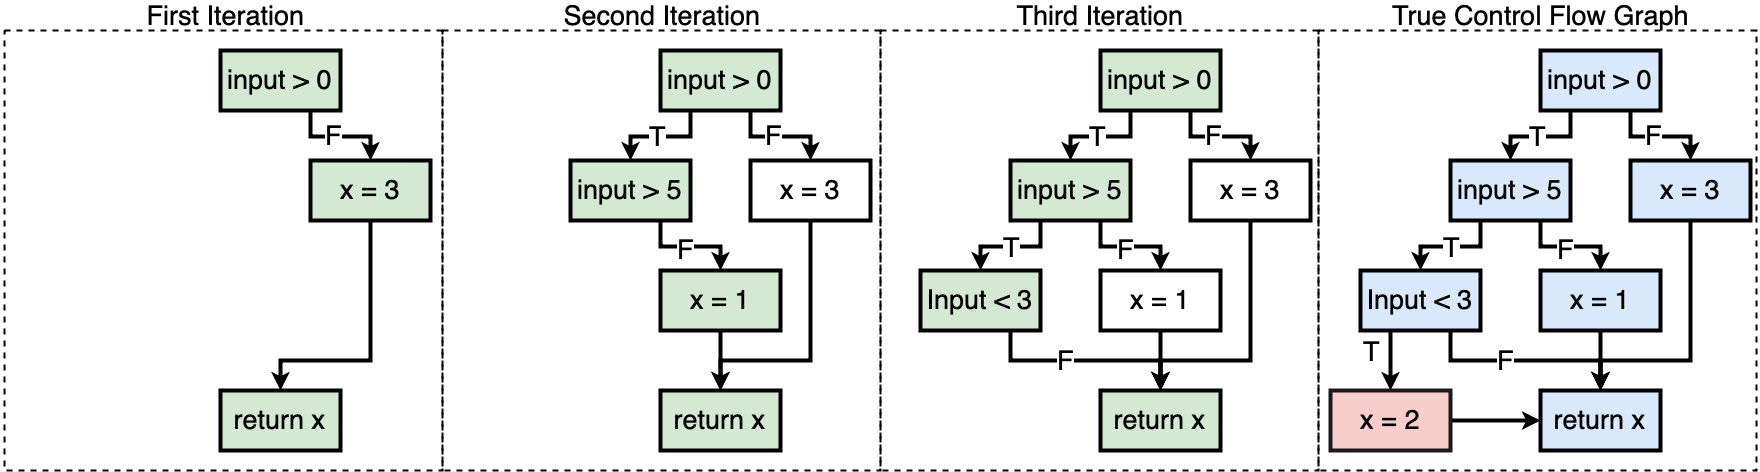
\includegraphics[width=\textwidth]{./images/cfg.png}
 \caption{The executed paths (shown in green) for each iteration of our study. The true control flow graph is depicted on the right with blue nodes depicting both nodes which our execution engine found and red nodes showing nodes which our execution engine found to be unsatisfiable.}
 \label{fig:cfg}
\end{figure*}

\section{Study}

Due to the scope of this project our main goal was to prototype this system to the point where feasibility could be shown. This study aims at showcasing this prototype while showcasing the design feasibility. The dynamic and static pass were crucial to the success of the concolic testing system. Thus both the dynamic and static LLVM pass were tested with the most common numeric data types namely:

\begin{itemize}
    \item Integers (32 bit and 64 bit)
    \item Floats (32 bit and 64 bit)
    \item Booleans (1 bit integers)
    \item Strings (8 bit integer pointers)
\end{itemize}

We also tested our LLVM passes on all of the statements which could cause branching such as if statements and loops. Interestingly, loops are handeled in the exact same way as if statements at a bitcode level. For example, consider Code Snippet~\ref{snip:loops}. The while loop was converted to an \textit{icmp} statement which is the same instruction type an if statement is converted to. Thus we later learnt that testing on both loops and if statements was actually redundant.

\vspace{-0.4cm}

\begin{lstlisting}[caption={Converting A Loop to Bit Code}, label=snip:loops]
Inst (icmp): %1 = icmp slt i32 %2, %3
Inst (br): br i1 %1, label %while.body, label %while.end
\end{lstlisting}

In order to prototype the system we implemented a constraint solver in Python using Z3. The constraint solver only handled integer values and was implemented in order to allow for a full run of the system which will discussed later in this section. 

We decided that fully automating the approach was not fundamental to showcasing the systems capabilities and thus only automated certain labour parts of the system. For instance, the process of automating the LLVM build, instrumentation, bitcode linking, and running of programs was done using shell scripts. The constraint solver was written in a single Python script and consumed trace files to automate the process of passing constraints to the solver. However in order to run a full test we manually generated traces and passed them to the solver which gave us input we manually passed back to the LLVM.

\subsection{Example Execution}

In this study, we go through an example using the program in code snippet~\ref{snip:prog}. To better understand how the execution works we also present Figure~\ref{fig:cfg} which shows which paths were executed during the concolic testing.

In our first run, we use the constraints solver to generate a random integer, which in our case was $-8361$ as seen in line 2 for Code Snippet~\ref{snip:step1}. We then run our program on this input and find that the only constraint we evaluate is $input > 0$ as seen in Code Snippet~\ref{snip:step1}. This input is evaluated as false, and there are no

\vspace{-0.6cm}

\begin{lstlisting}[caption={Original Program}, language=C, label=snip:prog]
int main(int argc, char **argv){
    int input = atoi(argv[1]);
    int x=0;
    if(input>0) {
        if(input > 5) {
            if(input < 3){
                x = 2;
            }
        }
        else{
            x = 1;
        }
    }
    else{
        x = 3;
    }
    return x;
}
\end{lstlisting}
\noindent
more predicates to evaluate on this path. Code Snippet~\ref{snip:step1} shows the system output for both the constraint solver and LLVM dynamic pass. We then pass the constraints from the LLVM trace to our constraint solver program, \texttt{solveConstraints.py}. This programs
negates the most recent un-negated constraint. In this case we negate the only constraint namely, !(input > 0). We then check if there is a satisfiable solution, which there is, and then generates new input.

\vspace{-0.6cm}

\begin{lstlisting}[caption={System Output - First Iteration}, label=snip:step1]
How many inputs values does this program take: 1
Your values are: [-8361]
=======================
Constraint Hit: input > 0
Operand (input): -8361 | Operand (0): 0
Predicate Evaluation: False
\end{lstlisting}

The new input which was generated was the value 1 as seen in line 1 of Code Snippet~\ref{snip:step2}.
On the second run, the program returns a trace saying that it evaluated two constraints upon execution, $input > 0$ as true and $input > 5$ as false. Each of these branches can be seen in the second iteration Figure~\ref{fig:cfg} as well as in the LLVM dynamic pass output in Code Snippet~\ref{snip:step2}. When we pass these constraints to our input generator, it negates $input > 5$ and generates the input of 6. 

\vspace{-0.6cm}

\begin{lstlisting}[caption={System Output - Second Iteration}, label=snip:step2]
sat - New Input: [a = 1]
========================
Constraint Hit: input > 0
Operand (input): 1 | Operand (0): 0
Predicate Evaluation: True
-----------------------
Constraint Hit: input > 5
Operand (input): 1 | Operand (5): 5
Predicate Evaluation: False
\end{lstlisting}

The third run, as seen in Code Snippet~\ref{snip:step3}, evaluates three constraints, $input > 0$ as true, $input > 5$ as true and $input < 3$ as false. We pass these constraints to our constraint solver with the last constraint, $!(input < 3)$, negated. Since input can not be both greater
than 5 and less than 3, this returns unsat. It is at this point that we have executed all paths in the control flow graph.

This ability to both stop after an unsat condition was found and consider flow senestive symbolic constraints is extremely useful. Consider for instance our static analysis LLVM pass whose results for the same original program are shown in Code Snippet~\ref{snip:static}. There is no way to tell which constraints are along the same branch, and the order in which these constraints are applied are unknown. 

\vspace{-0.6cm}

\begin{lstlisting}[caption={System Output - Final Iteration}, label=snip:step3]
sat - New Input: [a = 6]
========================
Constraint Hit: input > 0
Operand (input): 6 | Operand (0): 0
Predicate Evaluation: True
-----------------------
Constraint Hit: input > 5
Operand (input): 6 | Operand (5): 5
Predicate Evaluation: True
-----------------------
Constraint Hit: input < 3
Operand (input): 6 | Operand (3): 3
Predicate Evaluation: False
\end{lstlisting}

\vspace{-0.6cm}

\begin{lstlisting}[caption={System Output - Static Analysis}, label=snip:static]
Constraint: input > 0
Constraint: input > 5
Constraint: input < 3
\end{lstlisting}

Similarly our engines ability to determine that the constraints are unsat is extremely useful. Consider the case where path coverage is being used as a stopping condition for a random input fuzzer. The fuzzer would waste tons of execution trying to hit a branch which after only three executions of this approach was determined to be unsat.